\documentclass{article}

\usepackage{graphicx}
\usepackage{listings}
\lstset{language=C++}
\usepackage{hyperref}
\usepackage{amsthm}
\usepackage{lscape}
\usepackage{multirow}

\theoremstyle{remark}
\newtheorem{tutorial}{Tutorial }

\title{{\tt vle.extension.differential-equation} : simulation of 
ordinary differential equations into VLE.}

%%%%%%%%%%%%
\begin{document}

\maketitle

\tableofcontents

%%%%%%%%%%%%
\section{Introduction}

The package {\tt vle.extension.differential-equation} provides DEVS models
into VLE that allow the simulation of ordinary differential equation.


\section{Background theory}

Three methods are provided for numerical integration: Euler, Runge Kutta 4 and
QSS2 \cite{kofman.SIM02}. Euler and Runge Kutta 4 are well known explicit and
forward methods based on the discretization of the time. They are said to be 
time-slicing methods (TSM). QSS2 is also a forward and explicit method but it is
based on the discretization of variables, and developped especially for DEVS
models. For QSS2 implementation, the most general case is considered; 
ie. gradient expressions are non linear
functions depending on all state variables and thus :
\begin{itemize}
 \item gradient derivatives are computed numerically and not analytically as
 proposed for linear gradients.
\item quantization of variables involves an update of all variable gradients. 
\end{itemize}

Here, we focus on the strategies for handling
discontinuities into the systems and propose one strategy for VLE. These
discontinuities are the result of coupling discrete systems whith continuous
ones.

\subsection{State of the art: time events, state events}

Hybrid systems are defined as systems exhibiting both
continuous and discrete behaviors \cite{barros.ACM03}.
For numerical integration methods developper, 
these systems present the difficulty of handling discontinuities.
    
For Cellier and Kofman \cite{cellier.06}, discontinuities are 
discrete events and there exists two type of discontinuities :
\begin{itemize}
  \item state events. E.g. a ball that bounces the soil
   has a continuous behavior except at the time of contact 
   with the soil, at which the direction is changed. Equations 
   of the ball can be written whith \textit{switching function} 
   like in Dymola modeling environment, such as ~\\
   $y' = \textrm{ if } y < 0 \textrm{ then } -1 \textrm{ else } +1$
   \item time events. E.g. a control agent that takes decisions 
   on the conduct of a continuous system. 
\end{itemize}

One of the principal concern for handling state events is to detect them.
This can be achieved by using for example step-size control
\cite{esposito.ACM2007} and zero-crossing methods \cite{mao.CMA02}.
The family of QSSn methods \cite{cellier.SSIM08}
are well suited for handling state events since they 
rely on a discretization of state variable rather than discretization of time.
 
HFSS \cite{barros.ACM03} and DEV\&DESS \cite{zeigler.IMS06}
are formalisms that allow the simulation of hybrid systems.
DEV\&DESS rely on quantization methods and HFSS do not make assumptions 
on the integration method. It is not clear nevertheless how
 discontinuities are handled into these frameworks.  
 
For time events handling, no dedicated integration methods have been proposed,
only advises are given, as in \cite{cellier.06}.
If time events are scheduled (known in advance), step-size control can be
achieved in order to integrate over these events. In any case, the consequence
of a time event should be the beginning of a completely new integration,
that necesseraly starts with a re-initialisation of the system of differential
equations.

%Cellier and Kofman \cite{cellier.06} identify two sources of 
%discontinuity.

%- root finding solvers for state event : occurs with switching function
%models.

\subsection{Proposed strategy for time events management}
\label{sec:theory:strategy}

The strategy proposed for handling perturbations consists in reinitialising the
system of differential equation when a perturbation occurs as suggested
in \cite{cellier.06}. On perturbation, a propagation of the discontinuity is
performed into the system.

Figure \ref{fig:pertMgmt} is an example of the consequence of a
discontinuities into a system of differential equations. $S$ is a state variable
which gradient expression depends on variable $E$. At $t_p$, a perturbation on
state variable $S$ occurs and a discontinuity on $S$ is provoked. At $t_d$,
a discontinuity on variables $E$ occurs and provokes a discontinuity on the
gradient value of $S$.

\begin{figure}[!h]
\begin{center} 
\includegraphics[scale=1.4]{figures/perturbMgmt.pdf}
\caption{\label{fig:pertMgmt} Perturbations management strategy}
\end{center}
\end{figure}

On this example, the pertubation handling strategy is the following.
At time $t_2$, there is no perturbation yet and the numerical
integration processes as usual. 
Gradients computed at $t_1$ are used to compute the new value of $S$ and
a time step $\Delta_t = t_3 - t_2$ is provided for the duration of 
integration step. Into DEVS, this consists in calculating the time advance
function as $\sigma = \Delta_t$.

At time $t_p \in [t_2, t_3]$, a perturbation occurs on the model and the
following steps are performed:
\begin{itemize}
  \item[1] Update $S$ values at $t_p$  using a time step of value $t_p - t_2$.
  \item[2] Apply perturbation: reset the value of $S$ and his gradient.
  \item[3] Propagate a new discontinuity to variables that depends on $S$ in
  order to reinitialise them at $t_p$.
  \item[4] Compute the new $\sigma$ (in the figure, $\sigma = t_4 - t_p$)
\end{itemize}

At time $t_d \in [t_4, t_5]$, similar steps are performed, unless that
the discontinuity is propagated and not built:
\begin{itemize}
  \item[5] Update $S$ values at $t_d$  using a time step of value 
  $t_d - t_4$.
  \item[6] Apply discontinuity: reset the value of $S$ and his gradient.
  \item[7] Propagate a discontinuity to variables that depends on $S$ in order 
  to reinitialise them at $t_d$.
  \item[8] Compute the new $\sigma$ (in the figure, $\sigma = t_6 - t_d$)
\end{itemize}

Intuitively, a couple P-DEVS model that represents these systems 
are formed by a set of atomic models, each representing one variable.
In the case of a cycle of atomic models, e.g. when $S$ depends on $E$ and $E$
depends on $S$, using the strategy proposed will lead to discontinuities for
$S$ that are simultaneous ($t_d = t_p$) and an illegitimate P-DEVS model
\cite{zeigler.84} will be formed (ie. a infinite succession of bags with
$ta=0$) due to the propagation of discontinuity at $t_d$ (item 7).

To prevent this to happen, we build a discontinuity structure whith a message
$<iP,M_d>$ where $iP$ is an identifier of the perturbation and 
$M_d$ is the set of identifiers of models the perturbation passes through.
At time $t_d$, model $S$ propagates the discontinuity $<iP,M_d \cup
\{S\}> $ only if new models identifiers are present into $M_d$ for perturbation
$iP$.
On a system of differential equations of $n_v$ variables which is
perturbated by $n_p$ events at time $t_p$, the number of bags with $ta=0$ dedicated 
to reinitialisation will be in the worst case $n_v *
n_p * (n_v-1)$ and is finite. Indeed, the worst case is when each variable 
depends on all others variables of the system. Using this strategy, the P-DEVS
model is legitimate.


%%%%%%%%%%%%%%%
\section{User Documentation}

%%%%%%%%%%%%%%%
\subsection{Atomic model interface}
\label{sec:user:atomic}

\begin{figure}[!h]
\begin{center} 
\includegraphics[scale=0.80]{figures/userInterface.pdf}
\caption{\label{fig:userInt} The user interface of an atomic model.}
\end{center}
\end{figure}

Evolution of state variables $V_i$ is described by differential equation. 
These expressions can rely on the value of external variables $E_i$.
For time sclicing methods, external variables $E_i$  are expected to be
piecewise constant functions computed from continuous and derivable functions. 
For QSS2, external variables are expected to be
piecewise linear functions.

Atomic model ports $E_i$ and $V_i$ can carry data at time $t$ that contain:
\begin{itemize}
  \item 'name': the name of the external variable (or state variable)
  \item 'value': this is the value at $t$ of the variable 'name'.
  \item 'gradient' (optionnal): this is the value of the gradient of
  the variable 'name' at $t$.
  \item 'discontinuities' (the structure proposed in
  section \ref{sec:theory:strategy}): this should not be handled by the user.
\end{itemize} 
No other assumption, than continuity and derivability of the producing
function, is made regarding external variables updates. Particularly, updates of
$E_i$ variables can occur at any time.
   
Port 'perturb' can carry instant data (with no assumption on the producing
function) that is used to reset some state variables values. Reinitialisation 
of the state variables and their gradients is achieved by a function $reinit$
that the user can override. By default, the pertubation is interpreted as a  
reset of one state variable, and data must contain:
\begin{itemize}
  \item 'name': the name of the state variable targeted by the perturbation.
  \item 'value': the new value at of the state variable 'name'.
\end{itemize} 
Perturbations and discontinuities are handled by the formalism and do not
require special care of the user (see section \ref{sec:theory:strategy}) unless
perturbation is required to behave differently, in which case the function
$reinit$ should be proposed by the user.

%%%%%%%%%%%%
\subsection{Writing differential equations atomic models}
\label{sec:user:diff}

Below is given an example of dynamic for an atomic model that relies 
on the {\tt vle.extension.differential-equation}.

\begin{lstlisting}
class MyModel : public DifferentialEquation
{
public:
 MyModel(const DynamicsInit& model,
	     const InitEventList& events) :
    DifferentialEquation(model,events)
 {
 	//Initialisation of variables is done 
 	//into the class constructor:
	v = createVar("v");
	e = createExt("e");
 }
 
 //gradients of state variables are expressed 
 //into the 'compute' function 
 void compute(const Time& time)
 {
    	grad(v) = v() - e();
 }
 //Reinitialisation of state variables after a perturbation or 
 //a discontinuity is performed into the 'reinit' function
 //(optionnal)
 void reinit(bool isPerturb, const Value& message) 
 {
 }
 //states and external variables are attributes of the class
 Var v;
 Ext e;
};
\end{lstlisting}

%%%%%%%%%%%%
\subsection{Configuring atomics models into {\tt vpz} conditions}
\label{sec:user:conf}

The common structure of the conditions for configuring atomic models is the
following:
\begin{itemize}
  \item 'variables': a map that gives initialisation values of the
  state variables.
  \item 'method': the name of the numerical integration method to use for
  simulation ('rk4','euler' or 'qss2').
  \item 'method-parameters': a map that contains parameters of the specified
  method (see above).
\end{itemize} 

Three numerical integration methods are provided Runge Kutta 4 (rk4) Euler
(euler) and QSS2 (qss2). These are the parameters specific for each method.
\begin{itemize}
  \item For rk4 and euler:
  \begin{itemize}
    \item  'timestep' is a double value that gives the time step for
    integration.
    \item 'synchronisation' (optionnal) is a boolean. If true, integration steps
    are synchronized with external variables updates.
    \item output\_period (integer, default=1). It gives the period at which
    output of variable values are performed. They are output every
    ${output\_period} * {timestep}$ time unit.
  \end{itemize}
  \item For qss2: 
  \begin{itemize}
    \item 'DeltaQ' is a map that gives for each state variable the 
  quantum for integration.
	\item 'expect-gradients' (optionnal) is a boolean. If true, gradients are
	required for initialisation of state variables and external variables updates. 
  \end{itemize}
\end{itemize}

%%%%%%%%%%%%
\section{Technical details}

Some technical details are given below:
\begin{itemize}
  \item Description of the dynamic is based on DEVS state graph transition 
  and {\tt confluentTransition} implementation is used (see e.g. DEVS state
  graph for Time Slicing Methods implementation) 
  \item The base class {\tt DifferentialEquation} implementation is based,
  as far as possible, on the PIMPL idiom. Thus dynamics can be distinguished
  (eg. between QSS2 and Time Slicing Methods) and most of bugs corrections 
  would be stable regarding ABI.
  \item In an optimized use (no external variable and no perturbation), the
  integration step is ensured to be performed in only one bag.  
\end{itemize}


%%%%%%%%%%%%
\subsection{Global architecture}
\label{sec:archi}

\begin{landscape}
\vspace{-10cm}
\begin{figure}[!h]
\begin{center} 
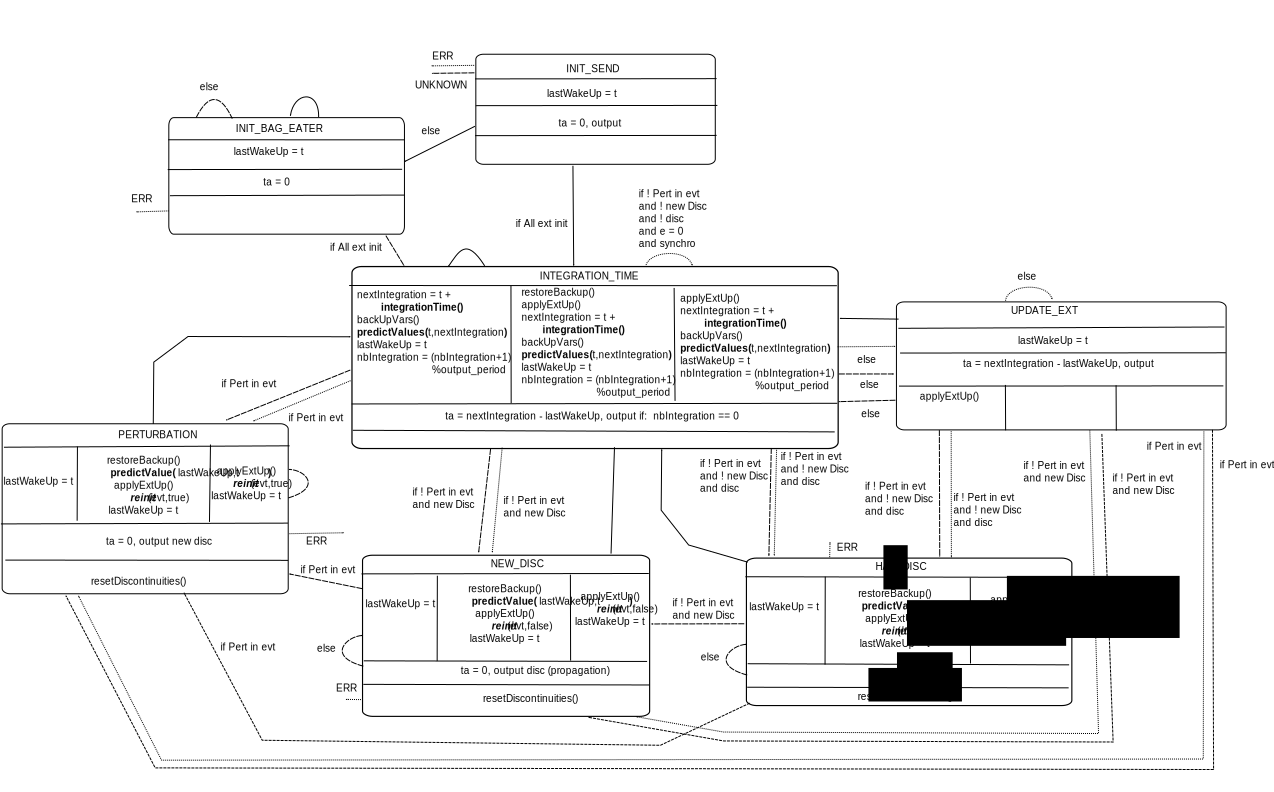
\includegraphics[scale=0.50]{figures/TimeSlicingDEVS.pdf}
\caption{\label{DEVSgraph} The DEVS state transition graph 
for Time Slicing methods (TSM).}
\end{center}
\end{figure}
\end{landscape}

%%%%%%%%%%%%
\subsection{Simulation time profiling}


Simulation time comparisons are based on the simulation of the Lotka Volterra
model and concern the three softwares VLE, powerdevs and R package deSolve. 
End time of simulation is set to 1500.
Two integration schemes are tested:
\begin{itemize}
  \item RK4 scheme with a time step of 0.01 (for deSolve and VLE)
  \item QSS2 scheme with a quantum value of 0.0001 (for powerdevs and VLE). Note
  that a lower quantum value results in a divergence process (and a $ta \to
  0$).
\end{itemize}
Different observations schemes are tested:
\begin{itemize}
  \item For VLE and powerdevs. A null observation which provides no output
  data.
  \item For VLE. A timed observation with a time-step of 0.01 and a 
  storage into a file.
  \item For VLE. A timed observation with a time-step of 0.01 and a 
  storage into memory. At the beginning, the matrix contains 
  10000 rows and is updated with 10000 more rows each time it is required to
  enlarge the matrix (these are the maximal values for VLE).
  \item For deSolve. A timed observation with a time-step of 0.01 and a 
  storage into a R matrix.
  \item For powerdevs. A plot using gnuplot of quantized values.
\end{itemize}


% \begin{tabular}{|c|c|c|c|}
% ~ & ~ & ~ & ~ \\
% \end{tabular}
\begin{figure}
\begin{center}
\begin{tabular}{|c|c|c|c|}
\hline
soft                      & observation         & RK4     & QSS2  \\\hline\hline
\multirow{2}{*}{powerdevs}& gnuplot             &  -      & 3.86  \\ \cline{2-4}
                          & null                &  -      & 0.76**  \\ \hline
deSolve                   & timed, mem. storage &  14.776* & -     \\ \hline
\multirow{3}{*}{VLE}      & timed, mem. storage &  6.468*  & 10.536\\\cline{2-4} 
                          & timed, file storage &  3.468  & 7.812 \\ \cline{2-4}
                          & null                &  1.072  & 4.824** \\ \hline
\end{tabular}
\caption{Comparison of time executions given in seconds.}
\end{center}
\end{figure}

\begin{figure}
\begin{center}
\begin{tabular}{|c|c|c|c|}
\hline
soft                      & observation         & RK4     & QSS2  \\\hline\hline
\multirow{2}{*}{powerdevs}& gnuplot             &  -      & 3.86  \\ \cline{2-4}
                          & null                &  -      & 0.76**  \\ \hline
deSolve                   & timed, mem. storage &  14.776* & -     \\ \hline
\multirow{3}{*}{VLE}      & timed, mem. storage &  0.74*  & 1.07\\\cline{2-4} 
                          & timed, file storage &  0.94  & 1.28 \\ \cline{2-4}
                          & null                &  0.1  & 0.37** \\ \hline
\end{tabular}
\caption{Comparison of time executions given in seconds. New TO BE
confirmed?!!.}
\end{center}
\end{figure}

Values quoted $(*)$ can be used to compare deSolve and VLE. This first
experiment shows better results for VLE. Moreover, VLE results should be 
improved if initialization size of the matrix is directly set to the final size
which is 150000 (rather than 10000). Values quoted $(**)$ can be used to compare
powerdevs and VLE and show clearly that powerdevs is faster.  



% LotkaVolterra (rk4, 0.01, 1500) ::
% deSolve :: 
%   utilisateur=14.761 systeme=0.000 ecoule= 14.776
% 
% LotkaVolterra (rk4, 0.01, 1500) :: 
% vle(without view) ::
%    1.072u 0.004s 0:01.08 99.0\% 0+0k 0+16io 0pf+0w
% 
% LotkaVolterra (rk4, 0.01, 1500) :: 
% vle(file view 0.01) ::
%    3.468u 0.036s 0:03.50 99.7\%	0+0k 0+24928io 0pf+0w
% 
% LotkaVolterra (rk4, 0.01, 1500) :: 
% vle(storage view 0.01 opt nrow=10000 updrow=10000) ::
% 	6.468u 0.068s 0:06.54 99.6\% 0+0k 0+16io 0pf+0w
%   
% LotkaVolterra (qss2, 0.0001, 1500) :: 
% powerdevs(gnuplot) ::
% 	3.86 secs
% 	
% LotkaVolterra (qss2, 0.0001, 1500) :: 
% powerdevs(without view) ::
% 	0.76 secs
% 
% LotkaVolterra (qss2, 0.0001, 1500) :: 
% vle(without view) ::	
% 	4.824u 0.008s 0:04.83 99.7\% 0+0k 0+16io 0pf+0w
% 		 
% LotkaVolterra (qss2, 0.0001, 1500) :: 
% vle(file view 0.01) :: 
% 	7.812u 0.020s 0:07.84 99.8\% 0+0k 0+24928io 0pf+0w
%   
% LotkaVolterra (qss2, 0.0001, 1500) :: 
% vle(storage view 0.01 opt nrow=10000 updrow=10000) ::
% 	10.536u 0.088s 0:10.63 99.8\% 0+0k 0+16io 0pf+0w


%%%%%%%%%%%%


% \begin{lstlisting}
% virtual const vv::Value& agent_start(
%                     const vv::Value& observation);
% virtual const vv::Value& agent_step(double reward,
%                     const vv::Value& observation);
% virtual void agent_episode_ends(double reward);
% virtual bool is_last_episode() const;
% \end{lstlisting}

\bibliographystyle{plain}
\bibliography{biblio}


\end{document}